\documentclass[10 pt,usenames,dvipsnames, oneside]{article}
\usepackage{../../../modelo-ensino-medio}



\begin{document}

\begin{center}
  \begin{minipage}[l]{3cm}

\includegraphics[width=2cm]{logo}    
\end{minipage}\hfill
\begin{minipage}[r]{.8\textwidth}
 {\Large \scshape Atividade: Próximo valor}  
\end{minipage}
\end{center}
\vspace{.2cm}

\ifdefined\prof
%Habilidades da BNCC
\begin{objetivos}
\item \textbf{EM13MAT304} Resolver e elaborar problemas com funções exponenciais nos quais é necessário compreender e interpretar a variação das grandezas envolvidas, em contextos como o da Matemática Financeira e o do crescimento de seres vivos microscópicos, entre outros. 
\end{objetivos}

%Caixa do Para o Professor
\begin{goals}
%Objetivos específicos
\begin{enumerate}
\item Reconhecer a função exponencial como modelo que apresenta maior crescimento em relação aos modelos afim e quadrático;
\end{enumerate}

\tcblower

%Orientações e sugestões
\begin{itemize}
\item Para ter uma maior variedade de exemplos no item (d) peça que cada estudante faça um diferente do que está no enunciado e que comparem uns com os outros.

\item No item (d), dependendo da escolha dos valores iniciais, pode ser que avaliar até $x=6$ não seja suficiente para concluir que a exponencial cresce mais. Caso isso ocorra, provoque os estudantes no sentido de extrapolar para valores maiores de $x$, e nesse caso, o uso de calculadoras gráficas é recomendado.

\item Uma construção feita no Desmos para explorar a construção dessa atividade \url{https://www.desmos.com/calculator/qtfjexncpo?lang=pt-BR}

\item Havendo possibilidade utilize esta construção \url{https://www.geogebra.org/m/GMvvpwrm\#material/CVMPHDfd} para explorar com a turma  as diferenças entre crescimento linear e exponencial.

\item Este outro link, explora como o crescimento exponencial supera os crescimento de funções polinomiais:  \url{https://www.geogebra.org/m/GMvvpwrm\#material/UfD3BXQa}
\end{itemize}
\end{goals}

\bigskip
\begin{center}
{\large \scshape Atividade}
\end{center}
\fi

Complete a tabela com os próximos valores de acordo com cada modelo especificado.

\begin{table}[H]
\centering

\scalebox{.9}
{
\begin{tabu} to \textwidth{|c|c|c|c|}
\hline
\thead
$\bm{x}$ & Afim & Quadrática & Exponencial \\
\hline
$0$ & $3$ & $3$ & $3$ \\
\hline
$1$ & $6$ & $6$ & $6$ \\
\hline
$2$ & & & \\
\hline
$3$ & & & \\
\hline
$4$ & & & \\
\hline
$5$ & & & \\
\hline
$6$ & & & \\
\hline
\end{tabu}
}
\end{table}

\begin{enumerate}

\item{}
Algum dos modelos é possível preencher de mais de uma forma? Qual(is)? Compare suas respostas com pelo menos dois de seus colegas.

\item{}
Admita que para o modelo quadrático o ponto $(0,3)$ é o vértice da parábola. Como preencher a coluna do meio nesse caso?

\item{}
Elabore expressões para cada um dos modelos (considerando o quadrático do item (b)) e use uma calculadora gráfica para representá-los e em um mesmo sistema de coordenadas.

\item{}
Qual dos modelos apresentou maior crescimento? Será que a sua resposta seria a mesma se trocássemos os valores iniciais (mantendo o mesmo para os três casos)?

\end{enumerate}

\ifdefined\prof
\begin{solucao}

Afim: 9,12,15, 18,21.

Quadrática: infinitas respostas (as diferenças devem ser PAs de segunda ordem).

Exponencial: 12, 24, 48, 56, 112.

\begin{enumerate}

\item Sim, o modelo quadrático.

\item $f(x)=kx^2+3$, e como $f(1)=6$, logo $k=3$: $15, 30, 51, 78, 111$.

\item $y=3+3x$, $y=3x^2+3$, $y=3\cdot 2^x$.

\begin{figure}[H]
\centering
\noindent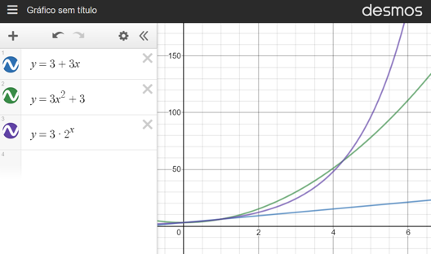
\includegraphics[width=250bp]{proximo_valor_itemC.png}
\end{figure}

\item Exponencial. A resposta se mantém, ou seja, a exponencial sempre vence.

\end{enumerate}

\end{solucao}
\fi

\end{document}